\chapter{Neural computation, formal languages and a direct reply to Chomsky}
\label{ch:learning-languages}
\reviewstatus{The constructive recurrence, finite causal-network representation, nonidentifiability example, and finite-family generalization bound are proved here. Transformer expressivity results and linguistic experiments are attributed external research. The argument rejects categorical impossibility claims; it does not turn a simulation theorem into a theorem about consciousness or a claim that a particular trained model generalizes without measurement.}

\section{The claim being challenged}

Chomsky's May 2023 interview makes two unusually strong claims: the design of large language models prevents them from contributing understanding of language or cognition as ``a matter of principle, irremediable'', and they ``work just as well with impossible languages'' \cite{LLchomskyMay}. These are stronger than the reasonable demand that a model of human language acquisition explain human learning constraints. They assert a principled barrier and a broad empirical equivalence. Neither follows from a neural architecture's use of prediction or from its ability to represent a large class of functions.

Our counterstance is direct: \emph{the categorical dismissal is wrong}. It conflates the objective used to train a model, the algorithms representable by that model, the algorithms actually learned, and the evidence required for a theory of human cognition. A predictive objective does not impose a theorem that internal mechanisms must be shallow, nonrecursive, or incapable of counterfactual computation. The appropriate response is to specify a model, prove what it can represent, inspect the mechanism it learns, and test its generalization under controlled interventions.

There is a valid distinction beneath the disagreement. A system can be a useful scientific instrument without being a faithful developmental model of a child. Its scientific value may lie in testing a proposed inductive bias, locating an internal representation, constructing a counterexample, or generating a checkable proof. We do not need to claim that every successful neural network is a correct biological theory in order to reject the assertion that such systems can contribute nothing in principle. Conversely, a claim about what a trained commercial model actually understands cannot be settled merely by selecting a sufficiently permissive mathematical definition of neural network.

The tensor-grammar framework makes these distinctions concrete. A graph grammar supplies a syntax. Its interpretation supplies denotational semantics. A recurrent or attention-based policy supplies a computational mechanism. Training supplies a procedure for choosing its parameters. A certificate verifies particular results. None of these levels is reducible to the others, but they can be composed into a system whose observable behavior has a precise semantic specification.

\section{A constructive recursive recognizer}

Let $D_1$ be the Dyck language with one kind of bracket. Encode an opening bracket by $+1$ and a closing bracket by $-1$. A word belongs to $D_1$ exactly when every prefix has nonnegative sum and the final sum is zero. Unlike a bounded collection of observed bracket strings, this is an unbounded language.

Write $\sigma(t)=\max(0,t)$ and
\[
 h(t)=\sigma(t)-\sigma(t-1).
\]
For an integer $t$, $h(t)=0$ when $t\le0$ and $h(t)=1$ when $t\ge1$. Consider the fixed recurrent update, with initial state $(c_0,e_0)=(0,0)$,
\begin{align*}
 c_t&=c_{t-1}+x_t,\\
 r_t&=h(-c_t),\\
 e_t&=\sigma(e_{t-1}-r_t)+r_t.
\end{align*}
The output is
\[
 a_t=\sigma\bigl(\sigma(1-|c_t|)-e_t\bigr),
 \qquad |c_t|=\sigma(c_t)+\sigma(-c_t).
\]
All operations are affine combinations and ReLUs. A signed intermediate value can be represented by its positive and negative parts if every hidden coordinate is required to be nonnegative.

\begin{theorem}[A fixed ReLU recurrence recognizes $D_1$]
\label{thm:relu-dyck}
Under exact integer arithmetic, the displayed fixed-size recurrent network outputs one exactly on the words of $D_1$ and zero on all other bracket words. On inputs of length at most $L$, its count requires $O(\log(L+1))$ bits.
\end{theorem}
\begin{proof}
Induction gives $c_t=\sum_{s\le t}x_s$. Hence $r_t$ is one exactly when the current prefix has negative balance. For binary $e,r$, $\sigma(e-r)+r=\max(e,r)$, so induction gives $e_t=1$ exactly when at least one prefix up to time $t$ is negative. Since $c_t$ is an integer, $\sigma(1-|c_t|)$ is one exactly when $c_t=0$ and is otherwise zero. The final ReLU therefore returns one exactly when $c_t=0$ and $e_t=0$, the defining condition for $D_1$. Finally $|c_t|\le L$, so a signed count has logarithmic bit length; the other recurrent state variable is binary.
\end{proof}

\begin{proposition}[Why the unbounded language is not regular]
$D_1$ is not recognized by any finite-state automaton.
\end{proposition}
\begin{proof}
It suffices to consider deterministic automata, since a nondeterministic finite automaton can be determinized using its finite subsets of states. If a deterministic automaton has $s$ states, two prefixes consisting of $i$ and $j$ opening brackets, $0\le i<j\le s$, reach the same state. Appending $i$ closing brackets must then produce the same acceptance decision for both. The first completed word is balanced and the second is not, a contradiction.
\end{proof}

This pair of proofs refutes a categorical assertion that a neural mechanism can only be a finite catalogue of shallow patterns. It also identifies the resource making the result possible: an integer count whose available precision grows with the input length. A fixed finite-precision device with bounded memory does not become an unbounded recognizer because the real-valued mathematical recurrence exists. The browser implements the exact recurrence for its bounded input field; the theorem describes the idealized family. Both descriptions are true at their respective scales.

The recurrence is constructed, not discovered by training. It therefore proves representability and supplies an executable specification. Whether a training method learns that algorithm from short examples, rather than a short-length shortcut, is a different experiment. A suitable test holds out longer lengths and deeper nestings, reports failure rates by depth, and compares states to the invariant $c_t=\sum_{s\le t}x_s$. Aggregate accuracy on the training length is inadequate.

\section{Transformer theorems require their hypotheses}

P\'erez, Barcel\'o and Marinkovic prove Turing completeness for a Transformer model with hard attention, positional encodings, and arbitrary-precision rational internal representations \cite{LLperez}. That theorem establishes a mathematical possibility under its specified model. It does not imply that a fixed-size softmax implementation with a fixed context window and hardware precision has unlimited memory, or that gradient descent finds the simulation.

Merrill and Sabharwal analyze intermediate decoding as a computational resource \cite{LLmerrill}. Their polynomial-step characterization uses logarithmic precision and, for the lower-bound construction, saturated attention, strict causal masking, and projected pre-normalization. Under those assumptions, polynomially many intermediate tokens suffice to capture polynomial-time computation. Their upper bounds also quantify the cost of shorter computations. These are external theorems, not results reproved or Lean-formalized in this companion.

Hahn's limitations for particular self-attention models remain part of the evidence \cite{LLhahn}. A limitation for one fixed-depth, fixed-resource model and a simulation theorem for a model with growing computational resources need not conflict. Nor does failure of one architecture prove impossibility for every neural network. Any argument that says only ``Transformers are Turing complete'' or only ``Transformers cannot handle recursion'' has omitted the variables on which the theorems depend.

The same discipline applies to a quantum ToricGT. A variational feature map can change a model's hypothesis class and its computational cost. It does not supply unbounded precision, an unlimited context window, or a proof of generalization. The new experiment trains an explicitly small circuit and measures its downstream performance. It is a defensible component study, not an inference that quantum hardware resolves the linguistic debate by itself.

\section{A neural circuit can compute a counterfactual}

The distinction between predicting an observation and answering an intervention is scientifically essential. It does not imply that neural arithmetic is intrinsically unable to represent an intervention. We can prove the contrary in a finite setting without relying on a universal approximation slogan.

For Boolean inputs $x_1,\ldots,x_m$, and a fixed pattern $b\in\{0,1\}^m$, define
\[
 I_b(x)=\sigma\left(\sum_{i:b_i=1}x_i+
                         \sum_{i:b_i=0}(1-x_i)-m+1\right).
\]
Every summand equals one exactly when the corresponding bit matches. Thus $I_b(x)$ is the exact indicator of $x=b$.

\begin{proposition}[Exact Boolean mechanisms in a ReLU network]
Every function $f:\{0,1\}^m\to\{0,1\}$ has the exact finite ReLU representation
\[
 f(x)=\sum_{b:f(b)=1}I_b(x).
\]
In particular, $x\wedge y=\sigma(x+y-1)$ and
$x\mathbin{\mathrm{xor}}y=x+y-2\sigma(x+y-1)$.
\end{proposition}
\begin{proof}
For Boolean $x$, exactly one pattern indicator is one, namely $I_x$, and every other one is zero. The sum therefore equals $f(x)$. Checking the four Boolean input pairs yields the two displayed special cases.
\end{proof}

\begin{theorem}[Finite structural counterfactuals have exact neural implementations]
\label{thm:relu-counterfactual}
Consider a finite acyclic structural causal model with Boolean endogenous and exogenous variables and specified deterministic Boolean structural functions. Given the exogenous assignment and a finite collection of interventions replacing selected structural functions by constants, a finite ReLU network computes all the resulting endogenous values exactly.
\end{theorem}
\begin{proof}
Topologically order the endogenous variables. Replace each structural function by the previous proposition's finite ReLU network, using its parents and exogenous variables as inputs. Composing in topological order computes the original model by induction. For an intervention indicator $i\in\{0,1\}$ and desired value $v$, replace an original Boolean output $f$ by
\[
 \sigma(f-i)+\sigma(v+i-1).
\]
If $i=0$ this is $f$; if $i=1$ it is $v$. Thus the same augmented network implements every chosen intervention mask. Reusing the same exogenous assignment across the original and intervened evaluations gives the structural counterfactual, with the replacement mechanism explicitly specified.
\end{proof}

This construction can be exponentially large in a mechanism's number of inputs. It proves capability, not universal computational efficiency. It also assumes that the causal mechanisms and the relevant exogenous state are supplied. Learning those from observations is a separate identifiability problem, exactly as emphasized in the causal-neural research of Xia and collaborators \cite{LLxia}. A mechanism written with ReLUs is still a mechanism. A neuron does not turn a structural intervention into a mere correlation.

\begin{proposition}[Observational ambiguity survives every learner]
There are two Boolean structural causal models with the same observational law for $(X,Y)$ and different laws for $Y$ under $\operatorname{do}(X=0)$. Consequently no procedure given only that observational law can always return the correct intervention law for both models.
\end{proposition}
\begin{proof}
Let $U$ be a fair Boolean variable. In the first model put $X=U$ and $Y=X$. In the second put $X=U$ and $Y=U$. Both observational laws assign probability $1/2$ to $(0,0)$ and $(1,1)$. Replacing the structural equation for $X$ by $X=0$ makes $Y=0$ surely in the first model, while in the second $Y=U$ remains fair. A procedure receives the same input law in both cases and so cannot be correct about two different output laws simultaneously.
\end{proof}

\begin{figure}[htbp]
\centering
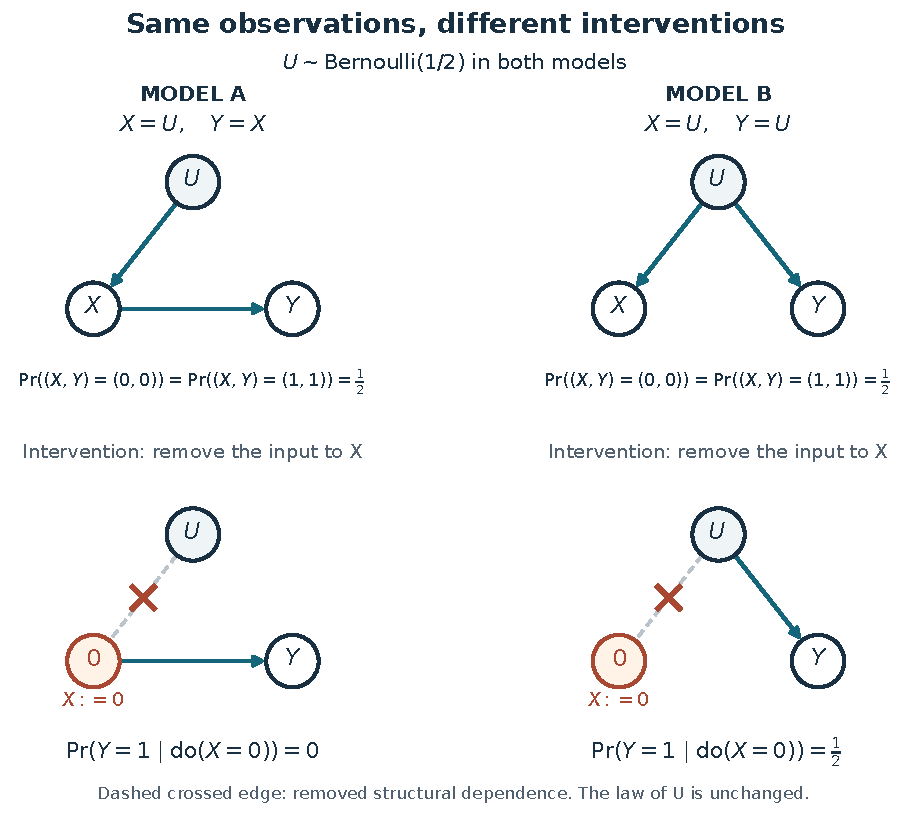
\includegraphics[width=\textwidth]{figures/second-pass-causal-models.pdf}
\caption{The same observational distribution does not identify a causal mechanism. Intervening on $X$ removes its incoming arrow. The two resulting laws for $Y$ differ even though the original observed $(X,Y)$ laws coincide.}
\label{fig:second-pass-causal}
\end{figure}

This impossibility applies equally to symbolic, neural, quantum, and human procedures with only those observations. It is an information limitation, not a defect peculiar to neural networks. Additional interventions, justified structural assumptions, or other observations can distinguish the models. The cosmology chapter uses precisely the same logic: a learned decoder cannot establish intentional cross-aeon communication if the proposed message and null hypotheses induce the same distribution on accessible observations.

The theorem also supplies a useful interpretation of ``understanding'' for this project. A system demonstrates a specified \emph{operational semantic competence} when it implements a model's interpretation map and answers its permitted transformations and counterfactual queries correctly. That is a testable property, with counterexamples and certificates. It does not settle phenomenal consciousness, the full semantics of natural language, or whether the supplied causal model is true of the world. Calling every such successful computation ``mere pattern matching'' adds no mathematical objection to its correctness.

\section{Empirical linguistic evidence and its strongest objection}

Gulordava and colleagues test long-distance agreement using semantically anomalous sentences and multiple languages, finding systematic syntactic generalization in recurrent language models \cite{LLgulordava}. Lakretz and colleagues identify internal units and circuits involved in number agreement and syntactic control \cite{LLlakretz}. These studies do not prove unlimited grammar mastery. They do provide concrete mechanisms and controlled behavior against which an assertion of exclusively superficial matching can be assessed.

Kallini and colleagues train GPT-2 variants on systematic transformations of English and observe differences in learning across their constructed languages \cite{LLkallini}. Their experiment challenges an unrestricted prediction of equal learning behavior. Hunter's subsequent critique identifies a serious confound: a central comparison adds a count-based nonadjacent dependency to one condition while leaving the other adjacent, instead of matching count-based and constituency-based nonadjacent dependencies \cite{LLhunter}. The experiment therefore does not settle whether the model's biases coincide with human grammatical constraints. Both findings belong in the assessment.

Comparisons between humans and language models also depend on the evaluation protocol. Lakretz and colleagues report a failure on particular long embedded dependencies \cite{LLnested}; Lampinen finds materially different performance when models receive prompts more comparable to the preparation supplied to human participants \cite{LLlampinen}. The appropriate conclusion is that instructions, examples, training distribution, and measured dependency type must be controlled. A benchmark failure is useful evidence about a defined setup. It is not an architecture-independent impossibility theorem.

For a stronger next experiment, construct pairs of synthetic grammars from one underlying set of annotated trees. Match vocabulary, sentence length, dependency distance, noise, and the number of extra transformation rules. Vary the grammatical relation of interest while keeping the nuisance quantities fixed or explicitly stratified. Train several architectures under matched data and optimization budgets; evaluate disjoint depths, vocabulary combinations, and intervention types. Compare test cross-entropy after accounting for the entropy of each data-generating process. Report counterexamples and uncertainty by stratum. This is a proposed experiment, not a result the present three-qubit graph benchmark has already established.

The hard counterstance does not require treating the weaker experiment as decisive. Chomsky's universal claim must itself meet a scientific burden. Demonstrated limitations and unresolved comparisons justify specific criticisms. They do not establish that neural models are permanently barred from representing mechanisms, learning useful linguistic structure, or contributing to explanations. Requiring an exact human developmental theory from every useful neural experiment mistakes one scientific question for all scientific questions about language.

\section{Learning a rule selector without surrendering guarantees}

Let $\mathcal R(G)$ be the finite set of certified grammar rules applicable to graph $G$. A model produces a probability distribution over this set. Its job may be to reduce a circuit's gate count, choose a template, propose a path, or select the next proof step. We can improve this proposal distribution while preserving a separate invariant checker. In particular, correctness of accepted semantic rewrites is independent of how they were ranked.

\begin{proposition}[A learned policy inherits certified rewrite correctness]
Suppose a system starts at a well-typed diagram, chooses any applicable rule according to an arbitrary, possibly history-dependent policy, checks the rule's stated semantic certificate, and accepts only certified rewrites. Every finite accepted run denotes the same map as its initial diagram.
\end{proposition}
\begin{proof}
Condition on any realized run. Each accepted step is a sound contextual replacement by Theorem~\ref{thm:typed-rewrite-soundness}. Induction on the finite number of accepted steps gives equal denotations. The policy's probabilities and parameters do not enter the argument.
\end{proof}

This is a substantive interface between learned and symbolic methods. The network can improve search order, while the checker enforces a property stated in mathematical terms. It does not make the checker unnecessary, and it does not make the learned component unimportant. Search cost can dominate a problem even when checking one proposed answer is easy. Whether a particular learned policy actually reduces that cost must be measured against a strong baseline with the same certificate budget.

For a quantum feature model, let $U_\theta(x)$ prepare a state and let $O_j$ be specified observables. Its classical feature vector has coordinates
$f_{\theta,j}(x)=\langle0|U_\theta(x)^\dagger O_jU_\theta(x)|0\rangle$.
These expectations are functions with a physical sampling cost and, for small circuits, an efficient classical implementation. A downstream model can use them to score graph rules. The model is therefore quantum in its feature construction when executed on quantum hardware, or a simulation of that construction when executed by cuQuantum or a CPU. A GPU state-vector simulation is a classical computation of a quantum model; this distinction is retained in the benchmark report.

\section{Finite-family generalization with an explicit selection cost}

A grammar can also generate candidate predictors. This introduces a statistical selection effect even if every candidate is mathematically well-typed. A small proof makes the cost visible.

\begin{lemma}[Bounded-variable exponential bound]
If $X\in[0,1]$ almost surely and $\mu=\mathbb EX$, then
$\mathbb E e^{\lambda(X-\mu)}\le e^{\lambda^2/8}$ for all real $\lambda$.
\end{lemma}
\begin{proof}
Let $\psi(\lambda)=\log\mathbb Ee^{\lambda X}$. Boundedness permits differentiation. Its second derivative is the variance of $X$ under the exponentially tilted probability measure. Any probability law supported on $[0,1]$ satisfies
$\operatorname{Var}(X)=\min_a\mathbb E(X-a)^2\le\mathbb E(X-1/2)^2\le1/4$.
Thus $\psi''\le1/4$, while $\psi(0)=0$ and $\psi'(0)=\mu$. Integrating this bound twice, or applying Taylor's theorem with integral remainder on the interval between zero and $\lambda$, gives
$\psi(\lambda)-\lambda\mu\le\lambda^2/8$.
\end{proof}

\begin{theorem}[Uniform error for a finite candidate family]
Let $K,m\ge1$ be integers and let $f_1,\ldots,f_K$ be predictors fixed independently of an independent identically distributed evaluation sample of size $m$. Let the loss lie in $[0,1]$, let $R_k$ be its population mean and $\widehat R_k$ its sample mean. For $0<\delta<1$, with probability at least $1-\delta$,
\[
 \max_{1\le k\le K}|\widehat R_k-R_k|
 \le \sqrt{\frac{\log(2K/\delta)}{2m}}.
\]
On this event the empirical minimizer's true risk is at most the best candidate's true risk plus twice this bound.
\end{theorem}
\begin{proof}
Independence and the exponential bound give
\[
 \mathbb E\exp\!\left(\lambda\sum_{i=1}^m(X_i-\mu)\right)
 \le\exp(m\lambda^2/8).
\]
Markov's inequality implies
$\Pr(\widehat\mu-\mu\ge\epsilon)\le\exp(-\lambda m\epsilon+m\lambda^2/8)$.
For $\lambda=4\epsilon$ this is $e^{-2m\epsilon^2}$; applying the same argument to $1-X$ gives the lower tail. A union bound over $K$ candidates yields $2K e^{-2m\epsilon^2}$. Solving for $\epsilon$ proves the displayed confidence bound. If $\hat k$ minimizes sample risk and $k_*$ minimizes true risk, then
$R_{\hat k}\le\widehat R_{\hat k}+\epsilon
\le\widehat R_{k_*}+\epsilon\le R_{k_*}+2\epsilon$.
\end{proof}

The independence condition matters. If the same evaluation data are repeatedly used to invent new predictors, the displayed proof no longer applies with the originally declared $K$. A finite family generated from a separate training sample can be conditioned on that sample and then evaluated on a fresh sample. More general adaptive selection requires another argument or a genuinely untouched final evaluation set. The cosmology chapter's global-null calibration addresses the analogous search over sky positions, template scales, and learned scoring rules.

This theorem does not certify the three-seed experiment merely because three is finite: the predictors are trained and selected, and their measured losses, splits, and boundedness must match its hypotheses. It supplies a reusable design rule. The reported benchmark uses explicit disjoint splits and exposes every seed; the finite-family theorem explains why tuning and final evaluation should be separated.

\section{What follows for the proposed cosmological grammar}

There are three layers in the proposed application. A physical model specifies how source degrees of freedom evolve through a crossover and into observable fields. A tensor grammar parameterizes candidate structures or messages consistent with that model. A learned function ranks or decodes those candidates using observed data. The second and third layers cannot establish the first by definition. They can make a specified physical hypothesis more testable.

One productive version is a restricted grammar of localized templates on an observed sky graph, with tensor-valued features for temperature, polarization, and angular correlations. A quantum feature map can feed an invariant graph scorer; a classical matched-filter or likelihood model supplies a strong baseline. The grammar's interface width determines a contraction budget. Null simulations must include the same mask, noise, foreground model, search over positions and widths, and learned model-selection procedure. Only held-out predictive success can establish that the search detected the stipulated class of signal better than its baseline. Attribution to a deliberate sender requires further, independently testable encoding structure.

At the logical level, the language of possible encoded messages can be regular, context free, or computationally more expressive depending on its stipulated encoder. Physics does not choose a Chomsky class merely by being quantum. A finite observed sky gives a finite dataset; an asymptotic language classification concerns a family of encoders and increasingly large observations. These are related through a specified model, not through the word ``information'' alone.

The same reasoning sharpens the reply to Chomsky. A neural system can participate in a disciplined semantic pipeline, can implement recursive and counterfactual algorithms, and can be evaluated on transformations that expose what it has learned. Demanding those tests is good science. Declaring the entire approach incapable of understanding in principle is not a consequence of the mathematical hierarchy, and is contradicted as a broad computational prohibition by the explicit constructions above. The unresolved question is which trained systems acquire which mechanisms, at what data and computational cost, with what robustness. That is an empirical and mathematical research program, not a reason to dismiss the program before doing it.
